\documentclass[a4paper]{article}
\usepackage{amsmath}
\usepackage{amsfonts}
\usepackage{amssymb}
\usepackage{graphicx}
\usepackage{float}

\begin{document}

\noindent \large Auteur: Siebe Haché \\
\noindent \large Studierichting: Informatica \\
\noindent \large Oefeningenreeks 5E nr. 3 \\

\medskip
\normalsize

Bereken de oppervlakte ingesloten door de hypocycloïde met parametervoorstelling:\\

$\left\{ \begin{array}{l} 
    x(t) = \dfrac{a}{3}(2 \cos t + \cos 2t)\\
    
    y(t) = \dfrac{a}{3}(2 \sin t - \sin2t) 
    
\end{array} \right. $\\

$S = \dfrac{1}{2} \left| \displaystyle\int_{0}^{2\pi} (x(t) \cdot y'(t) - y(t) \cdot x'(t)) \, dt \right|$\\

afleiden geeft:\\

$x'(t) = \dfrac{a}{3}(-2 \sin t - 2 \sin 2t) = -\dfrac{2a}{3}(\sin t + \sin 2t)$\\

$y'(t) = \dfrac{a}{3}(2 \cos t - 2 \cos 2t) = \dfrac{2a}{3}(\cos t - \cos 2t)$\\

$x \cdot y' - y \cdot x'$:\\

$\left[ \dfrac{a}{3}(2\cos t + \cos 2t) \cdot \dfrac{2a}{3}(\cos t - \cos 2t) \right] - \left[ \dfrac{a}{3}(2\sin t - \sin 2t) \cdot \left(-\dfrac{2a}{3}\right)(\sin t + \sin 2t) \right]$\\

$= \dfrac{2a^2}{9} \left[ (2\cos^2 t - 2\cos t \cos 2t + \cos 2t \cos t - \cos^2 2t) + (2\sin^2 t + 2\sin t \sin 2t - \sin 2t \sin t - \sin^2 2t) \right]$\\

$= \dfrac{2a^2}{9} \left[ 2(\cos^2 t + \sin^2 t) - (\cos^2 2t + \sin^2 2t) - (\cos t \cos 2t - \sin t \sin 2t) \right]$\\

$\Rightarrow \dfrac{2a^2}{9} \left[ 2(1) - (1) - \cos(t + 2t) \right] = \dfrac{2a^2}{9} (1 - \cos 3t)$\\

integraal: \\

$S = \dfrac{1}{2} \displaystyle\int_{0}^{2\pi} \dfrac{2a^2}{9} (1 - \cos 3t) \, dt$\\

$S = \dfrac{a^2}{9} \displaystyle\int_{0}^{2\pi} (1 - \cos 3t) \, dt$ \\

$S = \dfrac{a^2}{9} \left[ t - \dfrac{1}{3} \sin 3t \right]_{0}^{2\pi}$ \\

$S = \dfrac{a^2}{9} \left( (2\pi - 0) - (0 - 0) \right) = \dfrac{2\pi a^2}{9}$\\


\begin{figure}[H]
    \centering
    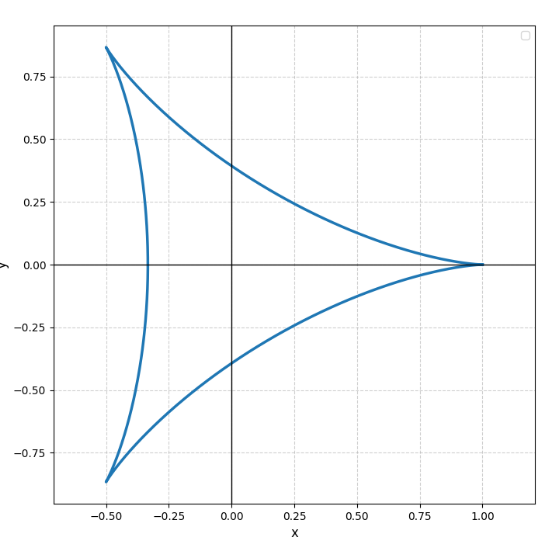
\includegraphics[width=0.6\textwidth]{5E-3-siebe.hache.INF.png}
\end{figure}

\begin{thebibliography}{999}
\bibitem{a} Grafiek gemaakt met Python
\end{thebibliography}
\end{document}